

\section{Modeling of signal and background processes}
\label{mcgeneration}

In this section we discuss the Monte Carlo generation of the signal and background
process samples used in this analysis.
%
We shall also discuss the modelling of detector
resolution effects.

\subsection{Higgs pair production in gluon-fusion}



Higgs pair production is simulated at leading order (LO) using
{\tt MadGraph5\_aMC@NLO}~\cite{Alwall:2014hca}.
%
We use a tailored  model~\cite{Maltoni:2014eza}
for gluon-fusion Higgs boson pair production
which includes mass effects
from the
exact form factors for the top-quark triangle and box
loops~\cite{Plehn:1996wb}.
%
Equivalent results can be obtained using
the recently available functionalities
for the calculation of loop-induced processes
in {\tt MadGraph5\_aMC@NLO}~\cite{Hirschi:2015iia}.
%
The calculation is performed in the
$n_f$=4 scheme,  accounting for  $b$-quark mass effects. 
The renormalization and factorization
scales are taken to be $\mu_F=\mu_R=H_T/2$,
with
\be
H_T\equiv \sum_i \sqrt{p_{T,i}^2+m_i^2} \, ,
\ee
the scalar sum of the
transverse masses of all final state particles.
%
For the input parton distribution functions (PDFs) we 
adopt the NNPDF 3.0 $n_f=4$ LO set~\cite{Ball:2014uwa} with
$\alpha_s(m_Z^2)=0.118$,
interfaced via {\tt LHAPDF6}~\cite{Buckley:2014ana}.
%
The Higgs boson couplings
and branching ratios are set to their SM values,
and its mass is taken to be
$m_h=125$ GeV~\cite{Aad:2014aba,Khachatryan:2014jba,Aad:2015zhl}.
%
In the SM, the Higgs trilinear coupling
is given by $\lambda=m_h^2/2v^2$, with
$v\simeq 246$ GeV the Higgs vacuum expectation
value.
%


%%%%%%%%%%%%%%%%%%%%%%%%%%%%
\begin{figure}[t]
\begin{center}
  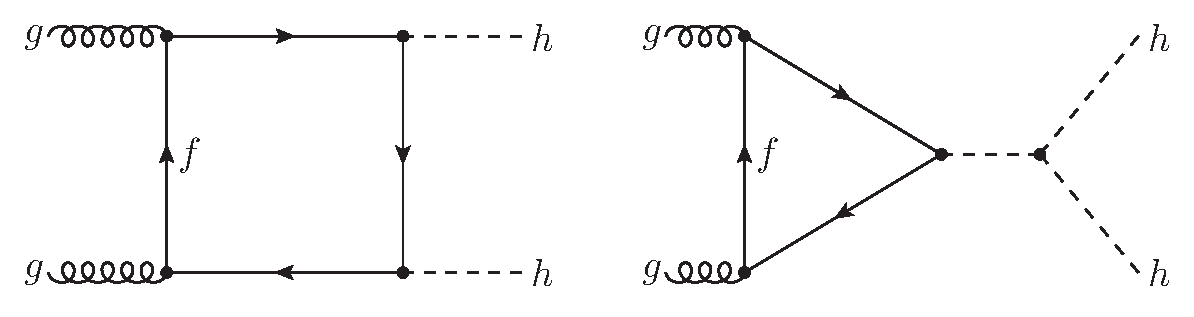
\includegraphics[width=0.96\textwidth]{plots/hhFeyn.pdf}
  \caption{\small Representative Feynman diagrams
    for Higgs pair production in gluon fusion at
    leading order.
    %
    Only the fermion triangle loop diagram (right) is
    directly sensitive to the Higgs trilinear coupling
    $\lambda$.
    %
    In the SM, the fermion loops are dominated by the
    contribution from the top quark.
}
\label{fig:hhFeyn}
\end{center}
\end{figure}
%%%%%%%%%%%%%%%%%%%%%%%


In Fig.~\ref{fig:hhFeyn} we show representative Feynman diagrams
    for LO Higgs pair production in gluon fusion.
    %
    The non-trivial interplay between the heavy quark box and the triangle loop diagrams
    can lead to either constructive or destructive interference
    and complicates the extraction of
    the trilinear coupling
    $\lambda$ from the measurement of the Higgs pair
    production cross-section.
    %
    Higher-order corrections~\cite{deFlorian:2013jea,Frederix:2014hta}
    are dominated by gluon radiation
    from either the initial state gluons or from the heavy quark loops.

    The total inclusive cross-section for this processes is
    known up to NNLO~\cite{deFlorian:2013jea}.
    %
    Resummed NNLO+NNLL calculations for Higgs pair production are
    also available~\cite{deFlorian:2015moa},
leading to a moderate enhancement of the order of
few percent as compared to the fixed-order NNLO calculation.
%
To achieve the correct higher-order value of the
integrated cross-section, we rescale our LO signal sample to match the
NNLO+NNLL
inclusive calculation.
%
This corresponds to
a $K$-factor $\sigma_{\rm NNLO+NNLL}/\sigma_{\rm LO}=2.4$, as indicated
in Table~\ref{tab:samples}.


Parton level signal events are then showered with the {\tt Pythia8} Monte
Carlo~\cite{Sjostrand:2007gs,Sjostrand:2014zea}, version {\tt v8.201}.
%
We use the default settings for the modeling
of the underlying event (UE), multiple parton
interactions (MPI), and PU, by means
of the Monash 2013 tune~\cite{Skands:2014pea},
based on the NNPDF2.3LO PDF set~\cite{Ball:2012cx,Ball:2013hta}.
%


\subsection{Backgrounds}

Background samples are generated at leading order
with {\tt SHERPA}~\cite{Gleisberg:2008ta} {\tt v2.1.1}.
%
As in the case of the signal generation,
the NNPDF 3.0 $n_f = 4$ LO set with strong coupling
$\alpha_s(m_Z^2)=0.118$ is used for all samples, and
we use as
factorisation and renormalisation scales $\mu_F=\mu_R=H_T/2$.
%
We account for the most relevant background
processes that can mimic the
 $hh\to 4b$ signal process.
%
This includes  QCD $4b$ multi-jet production, as well as
QCD $2b2j$ and $4j$ production, and top quark pair
production.
%
The latter is restricted to the fully hadronic final state,
since 
leptonic decays of top quarks can be removed by requiring
a lepton veto.
%
Single Higgs production processes such as $Z(\to b\bar{b})h(\to b\bar{b})$
and $t\bar{t}h(\to b\bar{b})$ along with electroweak backgrounds e.g $Z(\to b\bar{b})b\bar{b}$,
are much smaller than the QCD backgrounds~\cite{Wardrope:2014kya,deLima:2014dta}
and are therefore not included in the present analysis.
%



The LO cross-sections for
the background samples have been rescaled so that the integrated
distributions reproduce known higher-order QCD results.
%
For the $4b$ and $2b2j$ samples NLO/LO $K$-factors of 1.6 and 1.3
respectively have been determined
using {\tt MadGraph5\_aMC@NLO}~\cite{Alwall:2014hca}.
%
For the $4j$ sample, we rescale the LO cross-section
using the {\tt BLACKHAT}~\cite{Bern:2011ep}
calculation, resulting in
an NLO/LO $K$-factor of 0.6.
%
Finally, the LO cross-section for $t\bar{t}$ production has been rescaled
to match the NNLO+NNLL calculation of Ref.~\cite{Czakon:2013goa}, leading
to a $K$-factor of 1.4.
%
The $K$-factors that we use to rescale
the signal and background samples are summarised in
Table~\ref{tab:samples}.


 %%%%%%%%%%%%%%%%%%%%%%%%%%%%%%%%%%%%%%%%%%%%%%%%%%%%%%%%%%%%%%%
 %%%%%%%%%%%%%%%%%%%%%%%%%%%%%%%%%%%%%%%%%%%%%%%%%%%%%%%%%%%%%%%
\begin{table}[h]
  \small
\begin{center}
\begin{tabular}{|c|c|c|c|c|c|}
\hline
Process &  Generator & $N_{\mathrm{evt}}$ & $\sigma_{\mathrm{LO}}$ (pb)  & $K$-factor \\
\hline
\hline
$pp \to hh$ &  {\tt MadGraph5\_aMC@NLO} & 1M & $1.7\cdot10^{-2}$  &  2.4  (NNLO+NNLL~\cite{deFlorian:2013jea,deFlorian:2015moa}) \\
\hline
\hline
$pp \to b\bar{b}b\bar{b}$ &  {\tt SHERPA}v2.1.1 & 3M &$1.1 \cdot10^3$  & 1.6 (NLO~\cite{Alwall:2014hca}) \\
$pp \to b\bar{b}jj$ &  {\tt SHERPA}v2.1.1 & 3M & $2.7 \cdot 10^5$ & 1.3 (NLO~\cite{Alwall:2014hca}) \\
$pp \to jjjj$ &  {\tt SHERPA}v2.1.1 & 3M  & $9.7\cdot 10^6$ &  0.6 (NLO~\cite{Bern:2011ep})\\
$pp \to t\bar{t}\to b\bar{b}jjjj$ &  {\tt SHERPA}v2.1.1 & 3M & $2.5\cdot 10^3$   & 1.4 (NNLO+NNLL~\cite{Czakon:2013goa})\\
\hline
\end{tabular}
\caption{\small Details of the signal and background Monte
  Carlo samples used in this work.
  %
  For top quark production, only the hadronic final state is generated.
  %
  Also provided are the inclusive $K$-factors
  which are applied to reproduce the known
  higher-order results. \label{tab:samples}
} 
\end{center}
\end{table}%
%%%%%%%%%%%%%%%%%%%%%%%%%%%%%%%%%%%%%%%%%%%
%%%%%%%%%%%%%%%%%%%%%%%%%%%%%%%%%%%%%%%%%%%%%%%%%%%%%%%%%%%%%%%


At the generation level, the following loose selection 
cuts are applied to
background events.
%
Each final-state particle in the hard process must have $p_T \ge 20$ GeV, and be located
in the central  rapidity
region with
$| \eta | \le 3.0$.
%
At the matrix-element level
all final-state particles must also be separated by a minimum $\Delta R_{\mathrm{min}} =0.1$.
%
We have checked that these generator-level cuts are loose enough to have
no influence over the analysis cuts.
%
From Table~\ref{tab:samples}
we see that the $t\bar{t}$ and QCD $4b$ cross-sections are of
the same order of magnitude. However the former can be efficiently
reduced by using top quark reconstruction criteria.
%
The $bbjj$ cross-section is more than two orders
of magnitude larger than the $4b$ result, but will be suppressed
by the light and charm jet mis-identification rates,
required to contribute to the $4b$ final state.

 
 


As a cross-check of the {\tt SHERPA}
background cross-sections reported in Table~\ref{tab:samples}, we have produced leading-order
multi-jet samples
using {\tt MadGraph5\_aMC@NLO}, and
benchmarked them with the results for the same processes reported in
Ref.~\cite{Alwall:2014hca}.
%
For comparison with the latter numbers, 
we require that all samples include four anti-$k_T$ $R=0.5$ jets with $p_T \ge 80 $ GeV, where the leading jet must have $p_T \ge 100$ GeV, and with all jets within an acceptance of $|\eta| \le 2.5 $.
%
Using these common settings,
we find good agreement,
within the scale uncertainties, between the
{\tt MadGraph5\_aMC@NLO} and {\tt SHERPA} calculations of the multi-jet
backgrounds.


\subsection{Modelling of detector resolution}
\label{sec:detectormodeling}

While it is beyond the scope of this work to perform a full
detector simulation, it is important to include an estimate of detector
effects in the analysis, particularly for the finite energy
and angular resolutions which directly
degrade the reconstruction of important kinematical variables, such as
the invariant mass of the Higgs candidates.
%
Here we simulate the finite energy resolution of the ATLAS and CMS
hadronic calorimeters by applying a Gaussian smearing of the transverse
momentum $p_T$ with mean zero and standard deviation $\sigma_E$ for all
final-state particles before jet clustering, that is,
%
\be
\label{eq:smearing}
p_T^{(i)} \, \to \, p_T^{(i)\prime}= \lp 1+ r_i\cdot\sigma_E \rp\, p_T^{(i)} \, , \quad
i=1,\ldots,N_{\rm part} \, ,
\ee
with $r_i$ a univariate Gaussian random number, different for each
of the $N_{\rm part}$ particles in the event.
%
We take as a baseline value for the transverse momentum smearing a
factor of $\sigma_E=5\%$.
%

To account for the finite angular resolution of the calorimeter,
the $\lp \eta,\phi\rp$ plane is divided into regions of
$\Delta \eta \times \Delta \phi=0.1$, and each final state particle
which falls in each of these cells is set to the same $\eta$
and $\phi$ values of the center of the
corresponding cell.
%
Finally, the energy
of each final-state particle
is recalculated from the smeared $p_T^\prime$,
$\eta^\prime$ and $\phi^\prime$ values to ensure that the resulting
four-momentum is that of a light-like particle, since we neglect all
jet constituent masses in this analysis.


Our modelling of detector simulation has been tuned
to lead to a mass resolution of
the reconstructed Higgs candidates consistent
with the hadronic mass resolutions of the
ATLAS and CMS detectors~\cite{Aad:2012gxa,Chatrchyan:2013zna,Aad:2014xzb},
as discussed in Sect.~\ref{sec:pileup}.

%
